\chapter{Testes e análise de resultados}
	\label{ch:testes}
Nesta seção são discutidos os testes realizados com o \textit{software}, em seguida é comentado dos resultados obtidos. Os testes do sistema foram feitos durante testes do veículo do sub-sistema de suspensão monitorando dois elementos do veículo, uma célula de carga foi posicionada no \textit{link} superior esquerdo da suspensão traseira para aquisição dos dados da ação de forças sobre o mesmo e um sensor de temperatura foi acoplado ao cárter do motor para medir a temperatura do motor. Os outros sensores do veículo não foram abrangidos nos testes devido a não estarem prontos no período que os testes foram realizados. Alguns sensores são alterados entre o período de competição e precisam ser reimplementados no sistema. 

As Figuras \ref{fig:grafico_carga_parado}, \ref{fig:grafico_carga_andando} e \ref{fig:grafico_temperatura} exibem gráficos gerados pelo sistema em tempo de execução dos testes do veículo. É importante salientar que os valores dos gráficos recebidos pelos sensores não são importantes para este trabalho, o que é importante é o fato de que os valores estão condizentes com o que os sensores apresentam. Os dados exibidos são importantes para o projeto do sub-sistema de suspensão no caso do teste com a célula de carga e importantes para o sub-sistema do motor no caso da temperatura do motor. As conclusões dos testes são tiradas sobre os gráficos demostrados a seguir. Levando em conta que esta é a funcionalidade do sistema que melhor exemplifica seu funcionamento sem uma apresentação ao vivo do programa, as outras funcionalidade de demonstração dos dados em valores absolutos como a temperatura do motor demonstrada na Figura \ref{fig:telaprincipal} foram verificadas e funcionam em conjunto com os gráficos gerados. Consequentemente, é possível validar assim a demonstração dos dados em valores absolutos sem necessidade de impressão de um \textit{log} do programa.

 \begin{figure}[!htb]
	\center
	\caption{Gráficos gerados a partir de dados da célula de carga com o veículo parado.}
	\subfigure[Veículo parado no chão. Fonte: Elaborada pelo autor, 2018.]{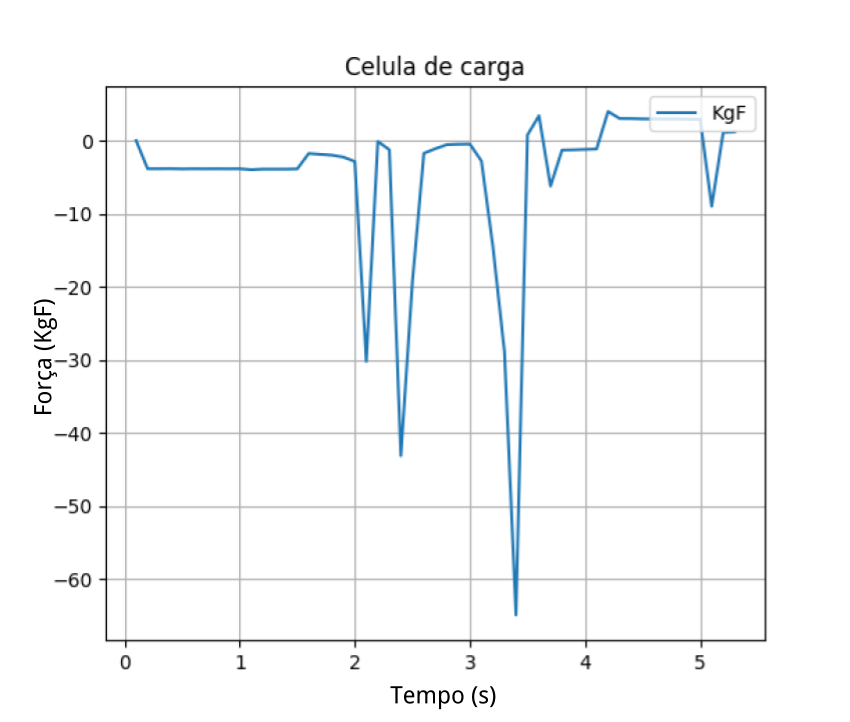
\includegraphics[width=7cm]{grafico_carga_chao}\label{fig:grafico_carga_chao}}
	\qquad
	\subfigure[Veículo parado com suspensão traseira suspensa. Fonte: Elaborada pelo autor, 2018.]{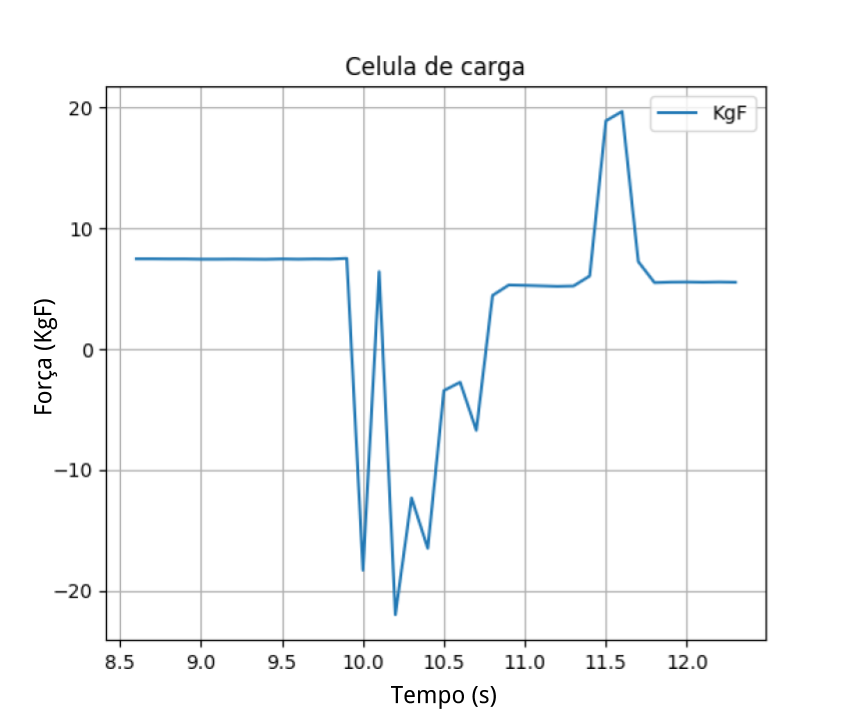
\includegraphics[width=7cm]{grafico_carga_levantado}\label{fig:grafico_carga_levantado}}
	\label{fig:grafico_carga_parado}
\end{figure}
     

\begin{figure}[!htb]
	\center
	\caption{Gráficos gerados a partir de dados da célula de carga com o veículo andando.}
	\subfigure[Veículo percorrendo a pista de testes no sentido horário. Fonte: Elaborada pelo autor, 2018.]{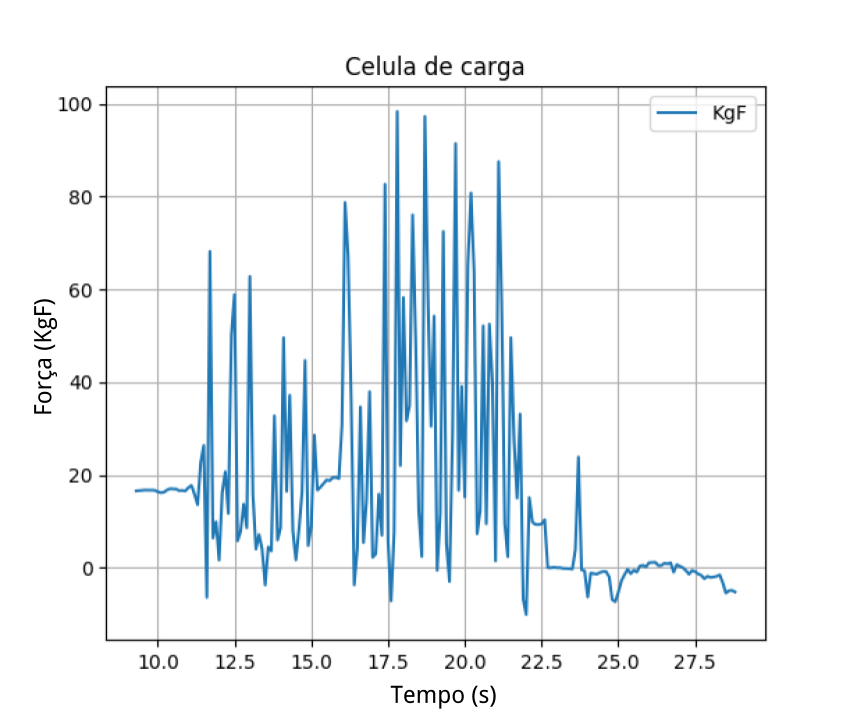
\includegraphics[width=6cm]{grafico_carga_volta1}\label{fig:grafico_carga_volta1}}
	\qquad
	\subfigure[Veículo percorrendo a pista de testes no sentido anti-horário. Fonte: Elaborada pelo autor, 2018.]{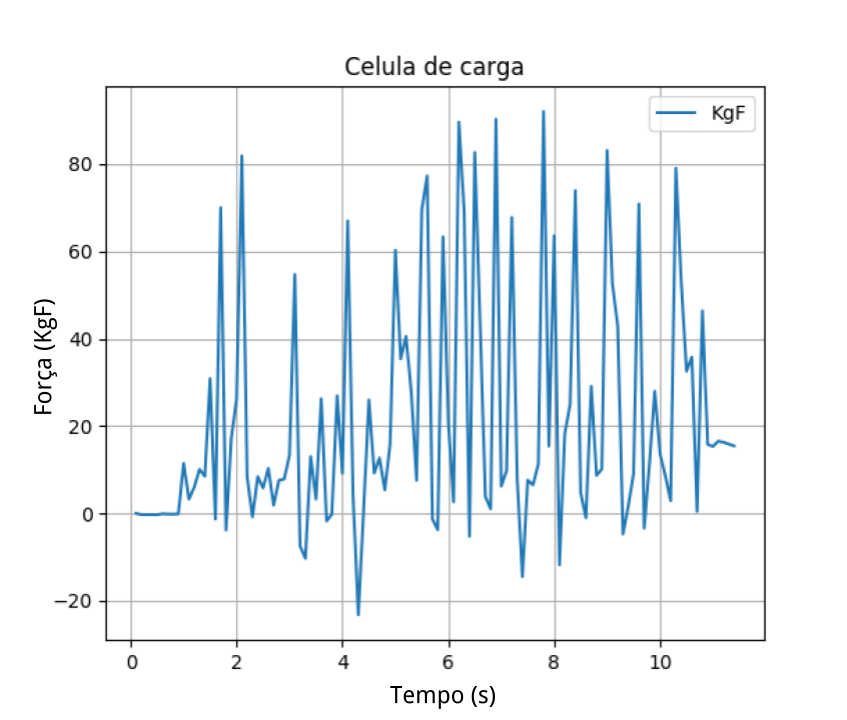
\includegraphics[width=6cm]{grafico_carga_volta2}\label{fig:grafico_carga_volta2}}
	\qquad
	\subfigure[Veículo percorrendo a pista em ritmo de corrida com saltos e tombo. Fonte: Elaborada pelo autor, 2018.]{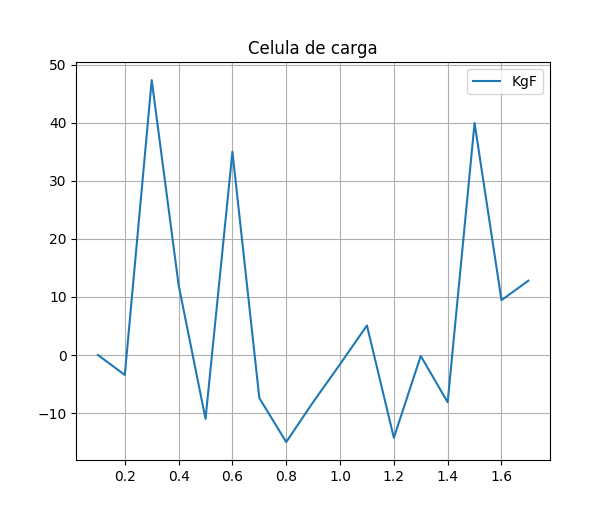
\includegraphics[width=6cm]{grafico_carga_tombo2corba}\label{fig:grafico_carga_tombo2corba}}
	\qquad
	\subfigure[Veículo andado em círculos. Fonte: Elaborada pelo autor, 2018.]{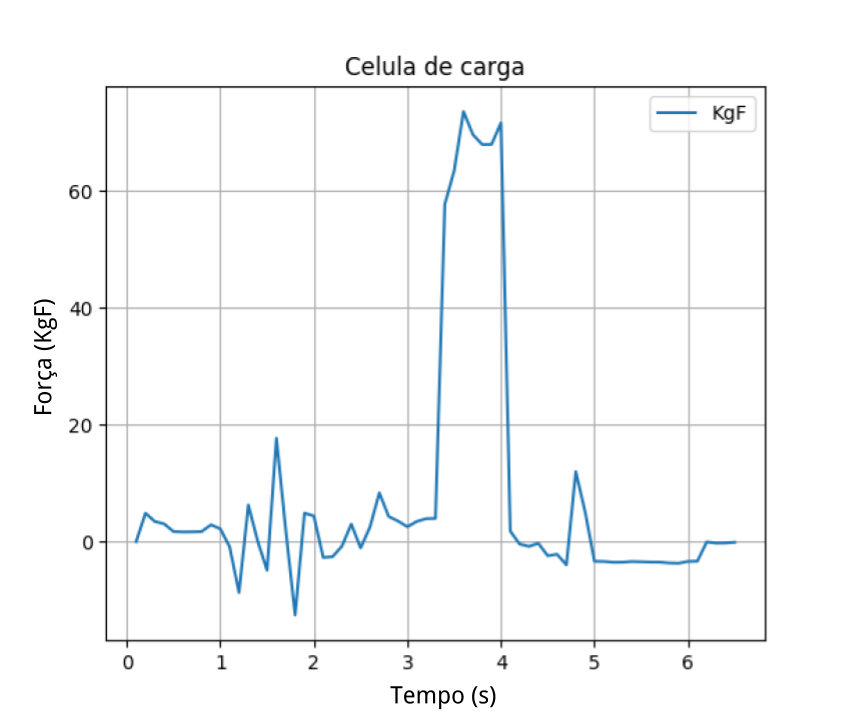
\includegraphics[width=6cm]{grafico_carga_zerinho}\label{fig:grafico_carga_zerinho}}
	\label{fig:grafico_carga_andando}
\end{figure}


 \begin{figure}[!htb]
	\center
	\caption{Gráficos gerados a partir de dados do sensor de temperatura.}
	\subfigure[Temperatura do óleo do motor no início dos testes. Fonte: Elaborada pelo autor, 2018.]{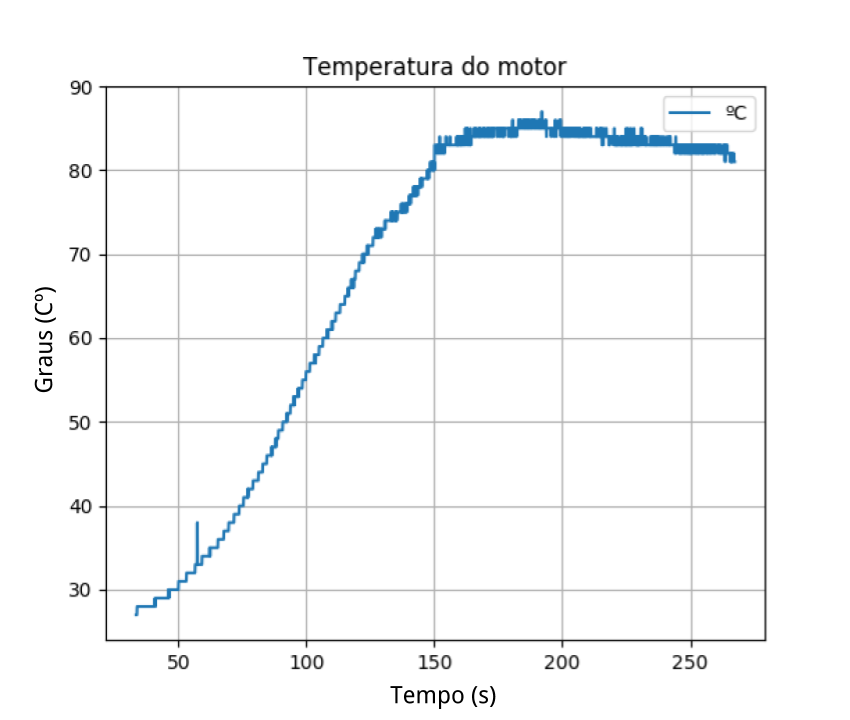
\includegraphics[width=10cm]{grafico_temperatura_inicio}\label{fig:grafico_temperatura_inicio}}
	\qquad
	\subfigure[Temperatura do óleo do motor do fim dos testes até entrada na oficina. Fonte: Elaborada pelo autor, 2018.]{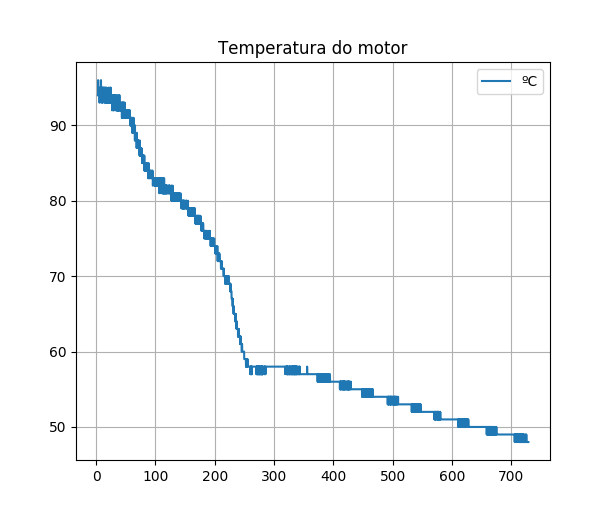
\includegraphics[width=10cm]{grafico_temperatura_final}\label{fig:grafico_temperatura_final}}
	\label{fig:grafico_temperatura}
\end{figure}

Os gráficos exibidos nas Figuras \ref{fig:grafico_carga_parado} e \ref{fig:grafico_carga_andando} indicam a força exercida sobre o \textit{link} superior esquerdo da suspensão traseira em quilograma-força no eixo vertical e o tempo em segundos no eixo horizontal. Os valores flutuam para números negativos quando o \textit{link} é comprimido e flutuam para números positivos quando o \textit{link} é tracionado. Os valores do eixo horizontal dados em segundos não estão corretos, isto se deve a alguns fatores explicados na Seção \ref{sec:taxa}. Já os gráficos exibidos na Figura \ref{fig:grafico_temperatura} indicam a temperatura do óleo do motor em graus Celsius no eixo vertical e o tempo em segundo no eixo horizontal. A verificação dos dados é explicada na Seção \ref{sec:validacao}. 

\section{Taxa de atualização}
\label{sec:taxa}

A taxa de atualização dos dados no sistema é definida pelo tempo em que os dados são atualizados do veículo para o computador. O sistema envia os dados de todos os sensores no mesmo pacote e isto se deve a limitação de recursos do projeto, pois a equipe Velociraptor possui apenas um par de módulos Xbee ZigBee S2/PRO S2. Devido a esta característica o sistema possui uma taxa de atualização do sistema de tratamento de dados igual a taxa de atualização dos dados do sensor com maior demora para atualizar. Alguns sensores possuem uma taxa de atualização dos dados mais rápida que a estipulada para o programa originalmente, nos testes realizados foi notado que o sensor de temperatura pode ser atualizado em até 100 milissegundos (ms) sem perda de informação, o que deixa uma margem para ajustar a taxa de atualização do mesmo, contudo também é notado que o sensor de célula de carga demora aproximadamente 2.000 ms para fazer os cálculos necessários para apresentar os dados na resolução escolhida.

Com estas informações é possível concluir que a taxa de atualização do sistema de tratamento de dados é igual a taxa de atualização do sensor de célula de carga. Com isto, a taxa de atualização é de uma atualização a cada 2.000 ms, um valor que não é satisfatório segundo a equipe dos boxes do Velociraptor. Porém, o sensor de célula de carga é utilizado apenas para testes e não deve entrar no veículo para provas de enduro ou provas de testes das competições do baja SAE. Portanto, os valores alcançados com o outro sensor testado de 100 ms são suficientes para a equipe. Testes futuros com os outros sensores do veículo devem manter ou negar esta taxa de atualização.

Outro fato que deve ser explicado é os valores em segundo dos gráficos apresentados nas Figuras \ref{fig:grafico_carga_parado}, \ref{fig:grafico_carga_andando} e \ref{fig:grafico_temperatura}. Devido a falta de conhecimento da real taxa de atualização dos dados do sensor da célula de carga, os valores aferidos para o sistema eram de 500 ms, no qual os segundos apresentados nos gráficos são escritos em 500 ms porém não são atualizados em 500 ms, mas sim em 2.000 ms. Este problema no código foi percebido durante a realização dos testes e não foi possível realizar novos testes com o código atualizado devido ao calendário de testes da equipe.

\section{Verificação dos dados}
\label{sec:validacao}

Para realizar a verificação da integridade dos dados apresentados nos gráficos, foram feitos testes em bancada com o sensor de temperatura do motor. Os testes foram realizados com o microcontrolador conectado a um computador, no qual os dados foram obtidos na porta analógica e após tratamento no microcontrolador eram mostrados na tela do computador conectado ao microcontrolador e também no sistema de tratamento de dados, que recebia os dados via ZigBee. 

Foram lidos alguns pacotes de dados do sensor em ambos os receptores e assim foi constatado que os dados não continham divergências, a mesma informação era encontrada em ambos. Os valores dos dados também foram comparados a distância, para verificar se o sistema quando fora do alcance entregava informações falsas. Foi constatado com o teste que as informações não são alteradas mesmo com a distância, elas apenas chegam com atraso ou dão \textit{timeout} como pode ser visto na Seção \ref{sec:distancia}.

\section{Distância de funcionamento dos módulos ZigBee}
\label{sec:distancia}

Um teste para medir a distância de funcionamento dos módulos foi realizado com o auxilio da ferramenta Google Maps. Este teste tinha um intuito de não apenas verificar as distâncias de funcionamento mas também de visualizar o comportamento do sistema quando utilizado no limite de seu alcance de operação. 

A distância anunciada \textit{indoor} ou em área urbana para os módulos Xbee Zigbee series 2 é de 40 metros e \textit{outdoor} ou em área rural é de 120 metros \cite{xbeeuserguide}. Os testes foram feitos em uma área urbana aberta em linha reta, e foram notados três tipos de comportamento nos módulos. Até 67 metros os dados eram enviados sem atraso e com consistência, até 94 metros os dados ainda eram enviados para o sistema de tratamento de dados porém alguns quadros chegavam com atraso de algumas centenas de milissegundos e a partir de 94 metros os dados não chegavam no sistema com consistência, levando a atrasos de diversos segundos. Os resultados mostram que a consistência de entrega é ainda maior que a declarada pelo fabricante, no momento dos testes os módulos estavam operando com tensão de 3.3V a recomendada pelo fabricante e testada com um multímetro. 

\section{Consumo de bateria}

Também foi feito um teste para descobrir o consumo de corrente da bateria adicionado no sistema. Este teste consistiu em ligar o SCOB sem o Xbee com a leitura do sensor de temperatura do motor e depois ligar o SCOB nas mesmas condições, porém com o Xbee. Ambos os sistemas estavam com o mesmo código no microcontrolador, rodando nas mesmas condições.

Então foi medido o uso de corrente em miliampere (mA) dos dois casos com um multímetro. No primeiro caso todo o SCOB consumia 22 mA e no segundo o valor saltou para 48 mA. Estes dados são coerentes olhando para os valores de consumo de corrente dados pelo fabricante no manual \cite{xbeeuserguide} e levando em conta que nem todas as funções do módulo estavam sendo utilizadas. A adição do Xbee foi a única mudança feita especificamente para o sistema de aquisição e tratamento de dados, além disto, esta mesma mudança já estava no escopo de projeto da equipe Velociraptor, o que indica que o aumento de consumo de corrente elétrica não deve causar grande impacto no sistema final.
